\documentclass[border=4pt]{standalone}
\usepackage{tikz}
\usetikzlibrary{arrows.meta,bending}
\begin{document}
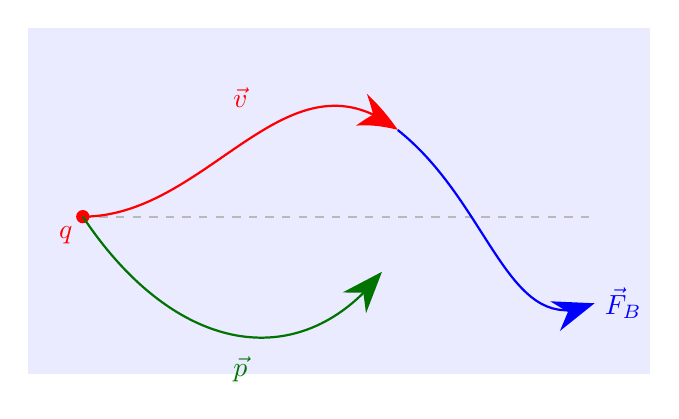
\begin{tikzpicture}[line width=.8pt]
  \fill[blue!8] (-.7,-2.0) rectangle (7.2,2.4);
  \draw[gray!55,dashed] (0,0) -- (6.5,0);
  \fill[red] (0,0) circle (2.4pt) node[below left] {$q$};

  \draw[red,-{Stealth[length=16pt,bend]}]
    (0,0) .. controls (1.6,0) and (2.6,2.2) .. (4.0,1.1);
  \draw[blue,-{Stealth[length=15pt,flex=.7]}]
    (4.0,1.1) .. controls (5.2,0.15) and (5.4,-1.6) .. (6.5,-1.1);
  \draw[green!45!black,-{Stealth[length=15pt,flex'=.75]}]
    (0,0) .. controls (1.2,-1.8) and (2.8,-2.0) .. (3.8,-.7);

  \node[red,above] at (2.0,1.25) {$\vec v$};
  \node[blue,right] at (6.5,-1.1) {$\vec F_B$};
  \node[green!45!black,below] at (2.0,-1.65) {$\vec p$};
\end{tikzpicture}
\end{document}
